\documentclass{subfiles}

\begin{document}

	

\section{Introduction}


\par To briefly summarise the previous sections, FW LiDAR data (Section \ref{AcquireData}) are laser scanning data particularly useful in Forestry, but the huge amount of information recorded make handling of the data difficult. The open source software DASOS (Section \ref{DASOS}) was developed along with this thesis to ease the usage of the data. DASOS voxelises (Section \ref{Voxelisation}) the data before interpretation and this approach is fundamentally different from the related, state-of-art software packages. The output of the voxelisation is a 3D discrete density volume. 

\par In order to visualise a voxel volume, it must be rendered in some form.  This chapter explains the process of reconstructing the surface of the scanned area from the 3D voxelised FW LiDAR. At first, volumetric rendering\footnote{Volumetric rendering refers the process of visualising 3D Volumes.} approaches are briefly explained in Section \ref{sec:RenderingApproaches}. Section \ref{sec:AlgebracObjects} gives a mathematical definition to the voxelised data, while Section \ref{sec:SurfaceReconstruction} describes the actual algorithm used to extract a surface. Finally, the results are given in Section \ref{sec:MCResults}. 


\section{Rendering Approaches of Volumetric Data}\label{sec:RenderingApproaches}
\par Even though the concept of visualising 3D discrete density volumes (Volumetric Visualisations) is new in forestry and remote sensing, it has been widely researched in medical imaging and visual effects. There are two approaches to visualising volumetric data.

\par The first approach is direct rendering, which repeatedly generates 2D images according to the view point (the camera). It is like "taking photos" {\color{red} *** Neill: Not sure about the analogy? Can you include a diagram from a papar or textbook to show what you mean?} from a camera and putting them in a sequence to produce an interactive video. An example of direct rendering approach is ray-tracing. Ray-tracing generates images by "taking photos"; rays are cast from the view point, passing through each pixel on a screen and carrying on into the volume.  Intensity values are assigned to the pixels according to the nearest intersections \cite{Hanrahan1983}. Ray-tracing can be time expensive depending on the complexity of the scene and, for that reason, some of the literature focuses on parallellising the ray-casting process. By introducing parallelisation, real time rendering of small volumetric data ($256^3$) was achieved by Pfister et al. in 1999 \cite{Pfister1999}. Also, after the release of the CUDA hardware \cite{Nickolls2008} (which is a parallel computing platform on recent nvidia graphics cards), Crassin et al. achieved real-time rendering of billions of voxels in 2009 \cite{Crassin2009}. 
	
\par The second approach is rasterisation, which is a method that maps primitive polygons (typically triangles) to pixels.  It is widely used in computer games, supported directly by common hardware acceleration systems and it is significantly faster than ray-tracing. Furthermore, interactive operations (e.g. measuring the distance between two trees) are trivial calculations on primitives/polygonal meshes and they are easy to implement.  In order to use this approach with volumes, they must be first converted to primitives.  This is commonly accomplished by surface reconstruction, referring to the extraction of a polygonal mesh, which is a set of primitives like triangles, from the volumetric data. Constructing a surface may take several minutes, but real time visualisations of polygonal meshes are supported by free animation packages (like Blender and Meshlab), in addition to being easy to implement.  So, even though it is possible to implement real-time interactive environments using direct rendering of the big voxel data, volumetric visualisation of FW LiDAR data is a new concept in remote sensing and, for simplicity, this thesis uses surface reconstruction.



\section{Algebraic Definition of the Volume}\label{sec:AlgebracObjects}

In computer graphics, objects can be defined using a function rather than being constructed from primitives. Those objects are called either implicit or algebraic. Implicit representation of objects enables a mathematical definition of the 3D discrete density volume generated from the FW LiDAR data (Section \ref{Voxelisation}). 

\par Algebraic objects were firstly introduced in computer graphics by Blinn in 1982 \cite{Blinn1982} to enable the definition of complex objects without saving a large amount of primitives; in some cases, primitives cannot accurate represent a shape (e.g. a sphere cannot be represented fully by a triangle mesh). Each object is defined by a function $ \mathit{f(X)} $ and the iso-surface value $\alpha$. The iso-surface value (iso-level) defines the boundaries of the object; for an object $ [f(x),a]$ every n-dimensional point $ \mathit{X} $  that lies on the surface of the object satisfies the condition $ \mathit{f(X)=\alpha }  $. To be more accurate, the following rules apply according to Pasko et al. \cite{Pasko1994}: 
\begin{itemize}
	\item $	\mathrm{f(X) = \alpha }$ , when $X$ lies on the surface of the algebraic object
	\item $	\mathrm{f(X) > \alpha }$ , when $X$ lies inside the algebraic object and
	\item $	\mathrm{f(X) < \alpha }$ , when $X$ lies outside the algebraic object	 
\end{itemize}

\par Regarding the algebraic representation of the 3D voxelised FW LiDAR data, X is a three dimensional point $\mathit{(x, y, z) }$ representing the longitude, latitude and height respectively and ${f(X)}$ is a function that takes  $\mathit{X}$ as input and returns the accumulated intensity value of the voxel that  $\mathit{X}$ lies inside. {\color{Fuchsia} Also, the iso-surface value $\mathit{\alpha }$ is a user defined parameter. Even though it closely related to the noise threshold used for filtering during voxelisation (Section \ref{Voxelisation}), it is different. The noise threshold filters low intensity samples before the volume is constructed, while the iso-surface value defines the boundaries of the object and it can be modified after the voxelisation because it doesn't affect the intensity values of the 3D voxelised FW LiDAR. Figure \ref{fig:SwitchingVisParameters} demonstrates how the iso-level parameter affects the output of the surface reconstruction of the voxelised FW LiDAR data in comparison to the noise filtering}.


\section {Surface Reconstruction with the Marching Cubes Algorithm}\label{sec:SurfaceReconstruction}

\par Even though numerical implicitisation is beneficial in reducing storage memory, visualising implicit objects is not straight forward, since they contain no discrete values. As described above in rendering volumes, this problem can be addressed either by direct rendering or surface reconstruction (Section \ref{sec:RenderingApproaches}). 

\par The Marching Cubes algorithm is an algorithm that polygonises implicit objects using a look up table. Let’s assume that $f(X)$ defines an implicit object. At first the space is divided into cubes. Each cube is defined by eight corner points and each corner point lies either inside or outside the implicit object. By enumerating all the possible cases and linearly interpolating the intersections along the edges, the surface of the implicit iso-surface is constructed \cite{Lorensen1987}. {\color{Fuchsia} The output is a polygonal mesh, a number of adjacent triangles constructed according to the user-defined iso-surface value $\alpha$  of the implicit object.
	
\par  The normals\footnote{ A normal is a vector that is perpendicular to the surface of a polygonal mesh. In graphics, the normals are important for calculating light illumination and each vertex is associated with one for smooth rendering of surfaces.} are calculated afterwards.} According to Lorensen and Cline \cite{Lorensen1987}, the normal of each vertex is calculated by measuring the local gradient change. Even though this work well on smooth object (e.g. a sphere defined by its equation), because of the high gradient changes in the voxelised FW LiDAR data this algorithm results into normals pointing into inconsistent directions. This is a problem because when the normals are not consistent, the surface of the object appears rough. For that reason, in DASOS the normal of each vertex is derived by the average normal of its adjacent triangles. 




\par Additionally it is worth highlighting that the sampling of the Marching cubes is independent from the sampling of the 3D density volume. But consistency between the two is required to avoid artefacts. Let’s assume the discrete volume has $(n \times m \times k)$ voxels, then the suggested sampling of Marching Cubes is $((n+1) \times (m+1) \times (k+1))$, as shown on Figure \ref{fig:MCSampling}; the black grid represents a 2D density grid and the blue grid represents the suggested sampling of the polygonisation. Please note that every point that lies outside the volume is considered to be outside the implicit object. {\color{Fuchsia} Figure \ref{fig:SamplingArtifacts} shows the effects of oversampling on a low resolution 3D density volume. On the right image the sampling of the volume appears as linear lines and squares on the forested areas because of the Marching Cubes' oversampling. Even though the right polygonal mesh looks blurred, it has been correctly sampled and the blur is because of the low resolution of the volume. Nevertheless there are no geometrical shapes on forested areas and once the resolution is increased then blur will disappear. }

    %% Sampling
    \begin{figure} [h!]
    	\begin{subfigure}[t]{.49\textwidth}
    		
    		\centering
    		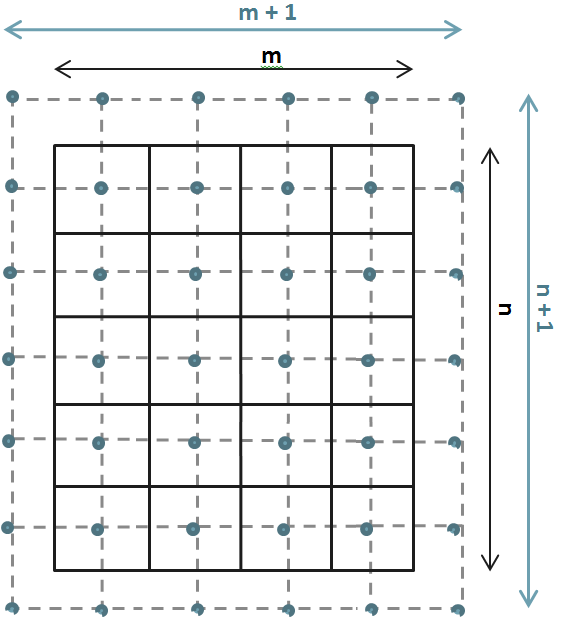
\includegraphics[width=.9\textwidth]{img/Sampling}
    		\caption{Suggested Sampling}
    		\label{fig:ExpectedSampling}
    	\end{subfigure} \hfill
    	\begin{subfigure}[t]{.49\textwidth}
    		\centering
    		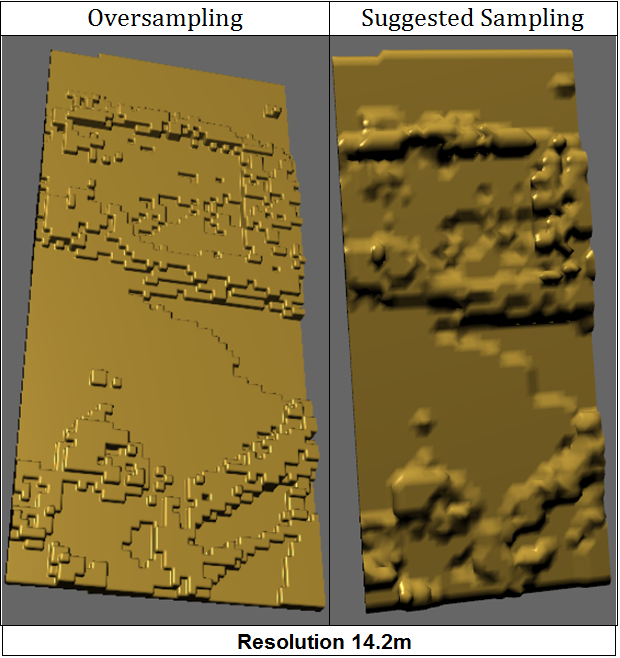
\includegraphics[width=.9\textwidth]{img/OversamplingVsSuggestedSampling}
    		\caption{Effects of Oversampling} 
    		\label{fig:SamplingArtifacts}
    	\end{subfigure} \hfill
    	\caption[Marching Cubes Sampling]{The suggested sampling during polygonisation using the Marching Cubes Algorithm}
    	\label{fig:MCSampling}
    \end{figure}


\section{Results}\label{sec:MCResults}

\par The output of DASOS is a polygonal mesh exported as an .obj file, which is a standard graphics format. The .obj files can be loaded into various animation software tools like Maya and Meshlab (Figure \ref{fig:AnimationPackages}). Figure \ref{fig:VariousFlightlines} shows polygonal meshes generated using NERC-ARF data from three different areas in the UK.  The region of interest is also user defined. The user defines whether an entire flightline or selected area is polygonised (Figure \ref{fig:SelectingRegionOfInterest}). 

\par Furthermore, there are three main user-defined parameters and Figure \ref{fig:SwitchingVisParameters} shows how the results are affected once modified:
\begin{enumerate}
	\item The voxel length controls the resolution of the output; the bigger the voxel length is the lower the resolution and the number of cubes are.
	\item The iso-level is the boundary that defines whether a voxel is inside or outside the implicit object. When the iso-level is increased, the number of voxels that are considered inside the implicit object decreases. For that reason, when it is too high most of the voxels are outside the boundary and the object seems to disappear.
	\item The noise level is the threshold of the low level filtering applied during voxelisation (Section \ref{Voxelisation}). If the noise level is too low, then the noise covers significant features of the data and when it is too high important information are discarded and the object seems to disappear again.
\end{enumerate}

 
\par Aside from computer-based visualisation, it is even possible to 3D print the meshes using something like MakerBot.  There are some difficulties as the meshes are not manifold\footnote{ A non-manifold polygonal object may have triangle below the outside surface of the object} (figure \ref{fig:3Dprinting}). Simplification of the mesh would have eased the processing of the .obj file in MakerBot. 
 

  
    \begin{figure} [h!]
    	\centering
    	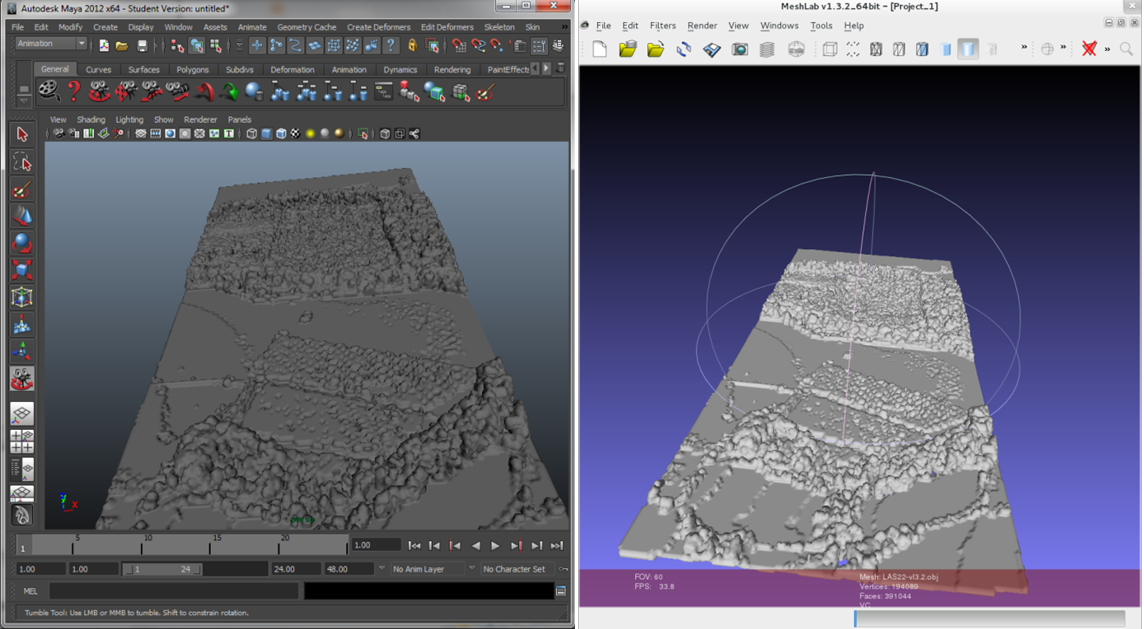
\includegraphics[width=0.9\textwidth]{img/AimationPackages.png}
    	\caption[Animation Packages]{Visualising the output of DASOS into animation software packages (Maya and Meshlab)}
    	\label{fig:AnimationPackages}
    \end{figure}
 
   \begin{figure} [h!]
   	\centering
   	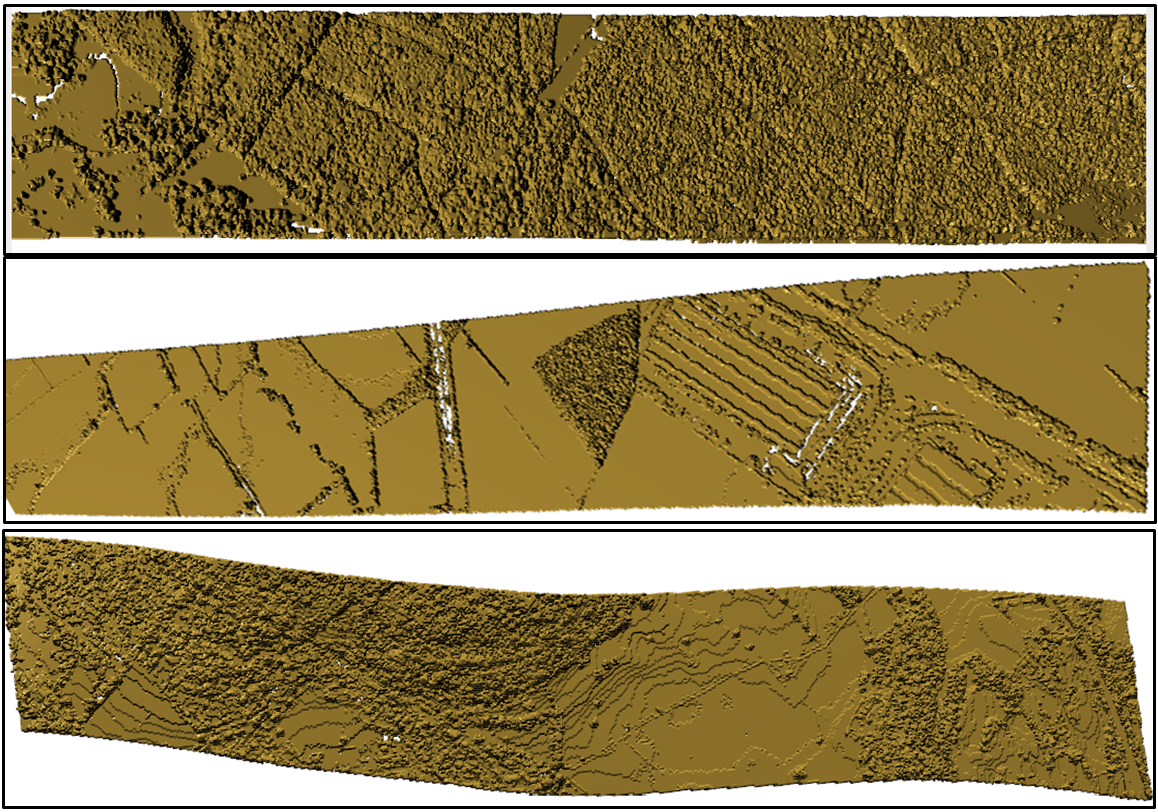
\includegraphics[width=.8\textwidth]{img/VariousFlightlines}
   	\caption[Various Flightlines Visualisation]{Polygonising NERC-ARF FW LiDAR data captured at different areas (New Forest, Milton Keynes and Eaves Wood)}
   	\label{fig:VariousFlightlines}
   \end{figure}

 \begin{figure} [h!]
 	\centering
 	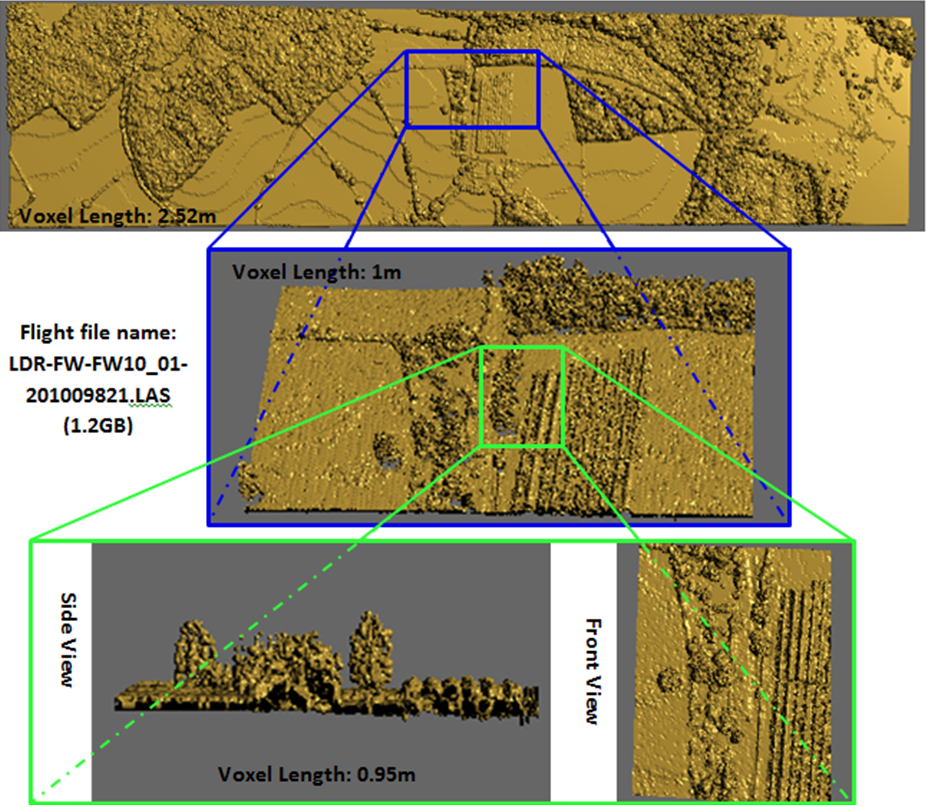
\includegraphics[width=.8\textwidth]{img/SelectingRegionOfInterest}
 	\caption[Selecting Region of Interest]{Selecting Region of Interest}
 	\label{fig:SelectingRegionOfInterest}
 \end{figure}
 

 

  

  
  \begin{figure} [h!]
  	\centering
  	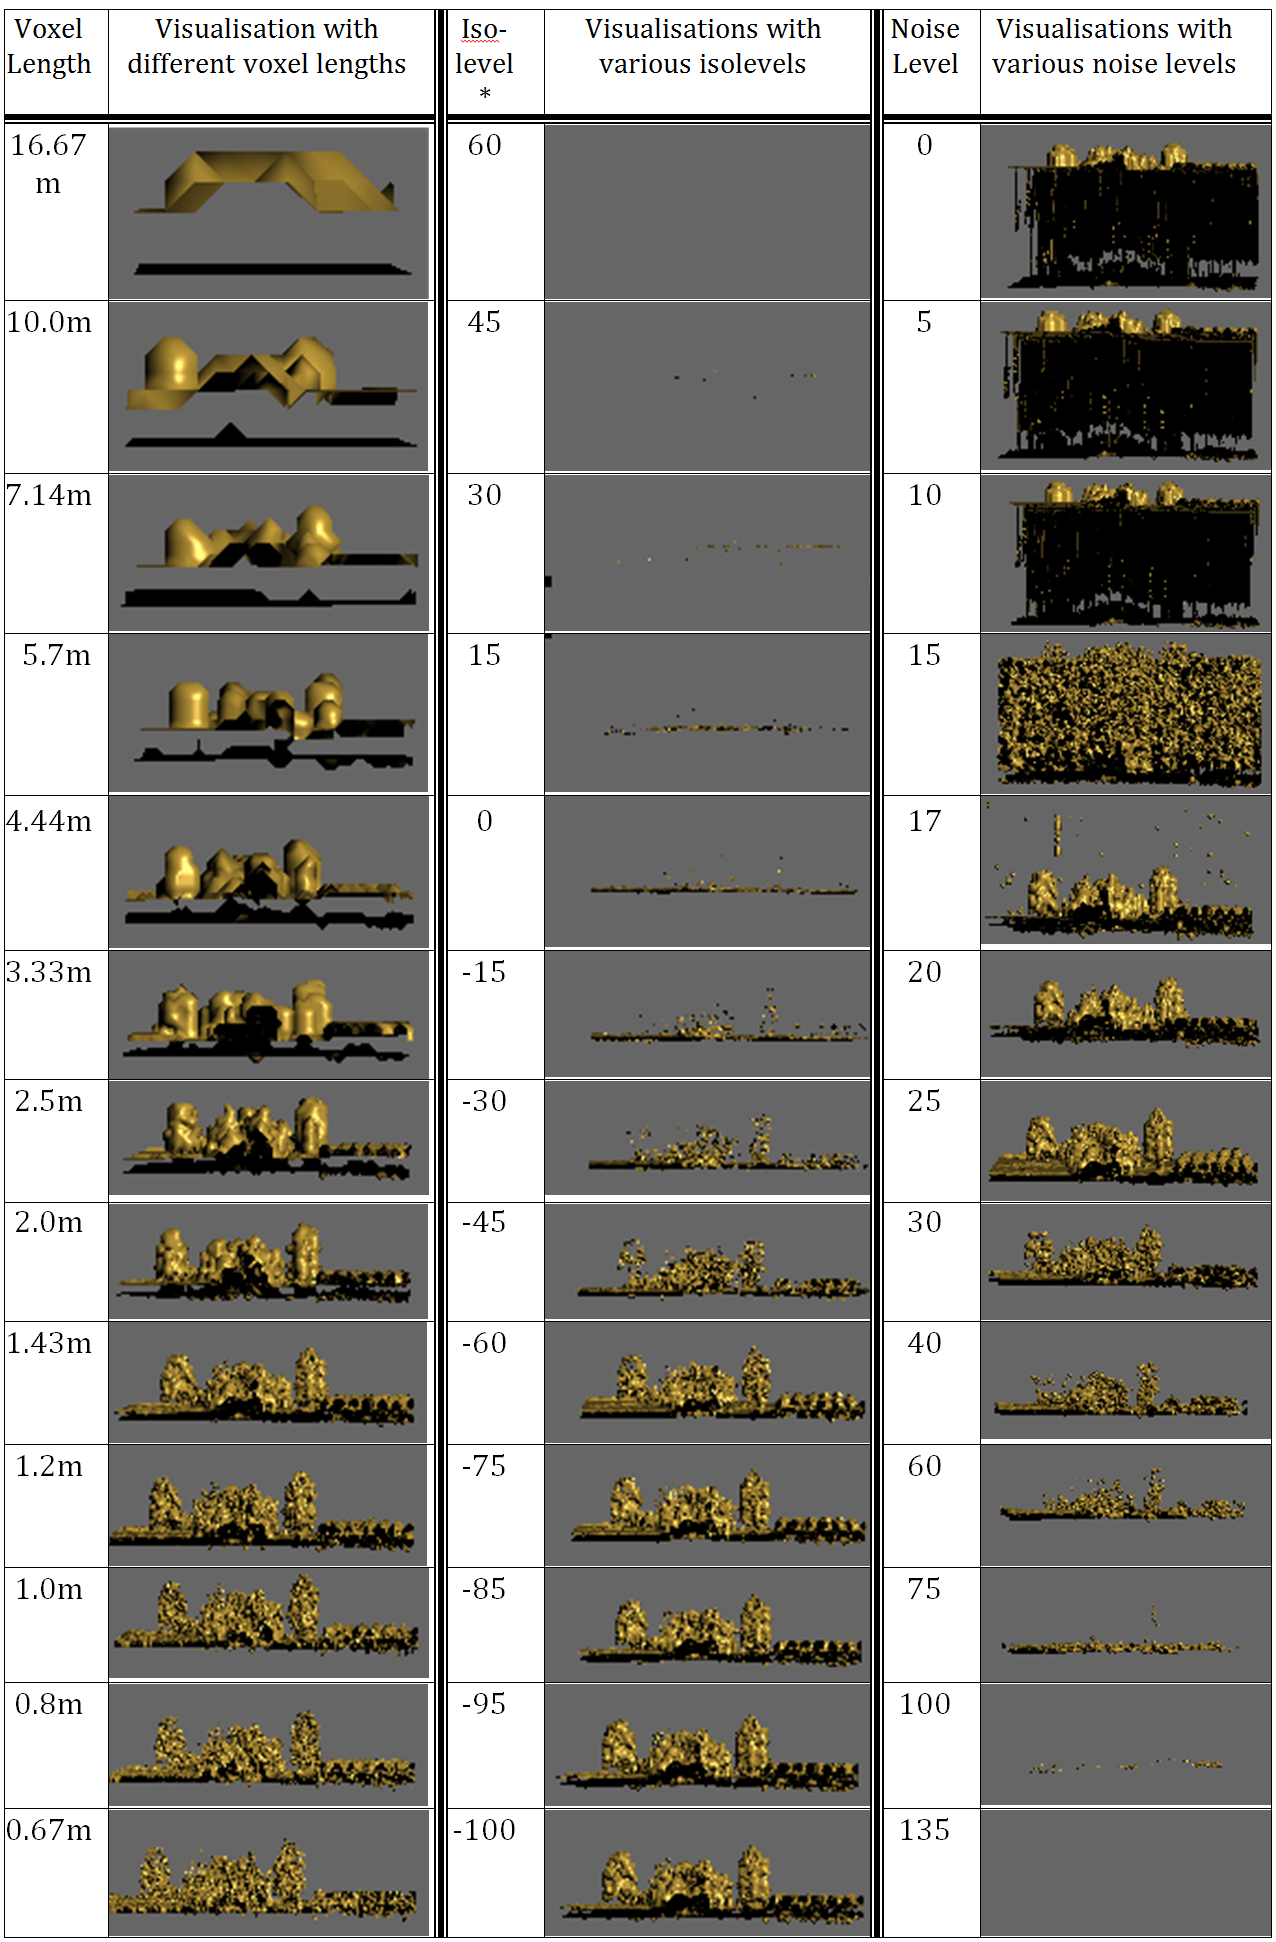
\includegraphics[width=0.91\textwidth]{img/SwitchingParameters}
  	\caption[Polygonisation Parameters]{How the output polygon mesh is affected by modifying the user-defined parameters (voxel length, isolevel\footnote{} and noise level). Please note that the intensities were scaled to be within the range [-100,100] and that the currently released version of DASOS does not scale the intensities.}
  	\label{fig:SwitchingVisParameters}
  \end{figure}
  

  
   \begin{figure} [h!]
   	\centering
   	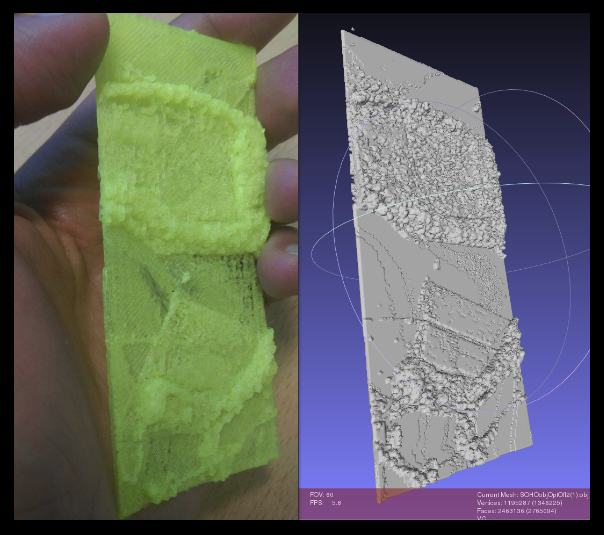
\includegraphics[width=0.9\textwidth]{img/NF-3Dprint}
   	\caption[3D printing]{3D printing of New Forest FW LiDAR data}
   	\label{fig:3Dprinting}
   \end{figure}

 

\end{document}
